% This is samplepaper.tex, a sample chapter demonstrating the
% LLNCS macro package for Springer Computer Science proceedings;
% Version 2.20 of 2017/10/04
%
\documentclass[runningheads]{llncs}
%
\usepackage{graphicx}
% Used for displaying a sample figure. If possible, figure files should
% be included in EPS format.
%
% If you use the hyperref package, please uncomment the following line
% to display URLs in blue roman font according to Springer's eBook style:
% \renewcommand\UrlFont{\color{blue}\rmfamily}

\begin{document}
%
\title{Direction-Free In-Air Signature Verification Using WIFI CSI Signal}
%
%\titlerunning{Abbreviated paper title}
% If the paper title is too long for the running head, you can set
% an abbreviated paper title here
%
\author{YoungWoong KWON\inst{1} \and
Jooyoung Kim\inst{1} \and
Kar-Ann Toh\inst{1}}
%
\authorrunning{Y. Kwon et al.}
% First names are abbreviated in the running head.
% If there are more than two authors, 'et al.' is used.
%
\institute{Yonsei University \and
\email{lncs@springer.com}\\
\url{http://www.springer.com/gp/computer-science/lncs} \and
ABC Institute, Rupert-Karls-University Heidelberg, Heidelberg, Germany\\
\email{\{abc,lncs\}@uni-heidelberg.de}}
%
\maketitle              % typeset the header of the contribution
%
\begin{abstract}
The abstract should briefly summarize the contents of the paper in
15--250 words.

\keywords{First keyword  \and Second keyword \and Another keyword.}
\end{abstract}
%
%
%
\section{Introduction}

\subsection{Motivation}
i. Pros of In-Air WIFI CSI signature system
1) Cheap: Use commercial device
2) Easy: No additional devices is needed
3) Secure: Hard to forgery
ii. Cons of In-Air WIFI CSI signature system
1) Setting direction problem
a) Different direction -> Different feature is needed
b) Hard to set exactly same direction as authentication before
Size of signature can varies

\subsection{Contribution}
- Overcome cons of WIFI signature system
- Robust to signal direction, size

\section{Related Works}

\subsection{ConvNets}
% description of convnet
Convolutional Neural Networks is a specal case of Multi Layer Perceptron and it has unified feature extractor and classifier in one network. It has been widely applied to visual objects such as image, video or 2D array input. Several factors make ConvNets attractive in image related tasks.
Local connectivity captures local correlation property of image. It is applycable by using ConvNet filter.Weight sharing helps to reduce the number of weights in feature maps.
Also, CUDA libraries makes the tranining feature maps easier to reduce training time.
%

\subsection{Siamese Networks}

% history of siamese net
In \cite{bromley1994signature}, LeCun et al. Introduced Siamese nets as parts of their handwritten signature verification system. 
A siamese neural network consists of twin networks which accept distinct inputs but are joined by an energy function at the top.\cite{koch2015siamese}

% description of siamese net
% from https://becominghuman.ai/siamese-networks-algorithm-applications-and-pytorch-implementation-4ffa3304c18

It is important that not only the architecture of the subnetworks is identical, but the weights have to be shared among them as well for the network to be called “siamese”.
Usually, siamese networks perform binary classification at the output, classifying if the inputs are of the same class or not

% end site


% differences in feature extractor
They proposed a feature extractor based on Time Delay Neural Networks\cite{lang1990time} and feature matcher based on cosine distance of feature vector. 





% another research which used Siamese Nets
In a recent related study, pedestrian tracking \cite{Leal-Taixe_2016_CVPR_Workshops}, object cosegmedtation \cite{mukherjee2018object} showed that Siamese Networks can be used for image classification tasks and \cite{maheshwary2018matching} captures semantics from job resumes.


\section{Proposed System}

In this section, we propose a direction-free identify verification system based on the Wi-Fi based in-air handwritten signature (will be called Wi-Fi signature signals hereafter). An overview of the proposed system utilizing the Siamese network learning is shown in Fig.1.
Essentially, the Wi-Fi signature signals are preprocessed to create the input data for our Siamese network. Subsequently, the Siamese network using ConvNet structure is trained to measure the similarity between two inputs. The resultant similarity score is utilized to verify whether the input signals are belong to the same identity regardless of the capturing directions. The following subsections detail the
data preprocessing and the Siamese network model.

% Figure 1
\begin{figure}
    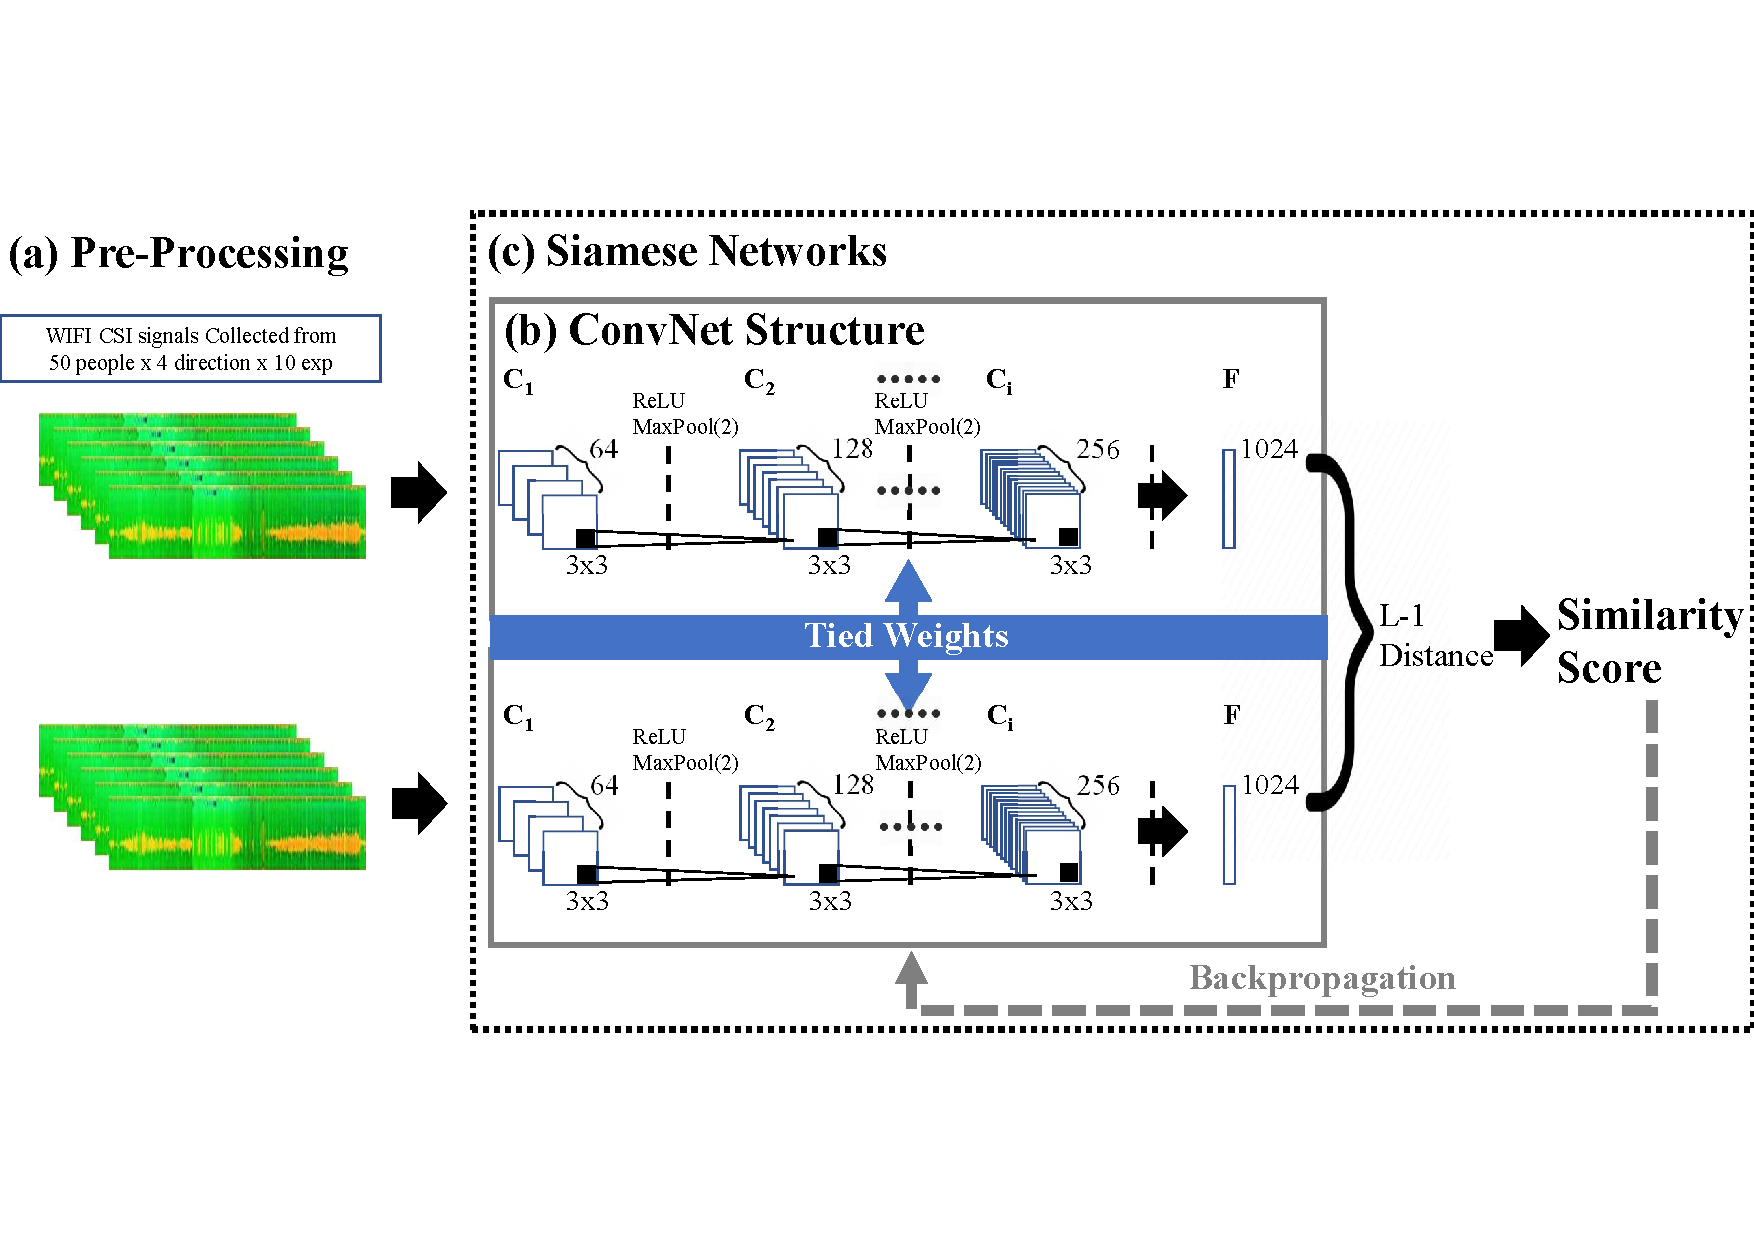
\includegraphics[width=\textwidth]{network3.pdf}
    \caption{Structure of Siamese network} \label{fig1}
\end{figure}

\subsection{Data Preprocessing}

Since every Wi-Fi signature signal has different data size, we firstly adopted the gradient operation with respect to the time instance to measure the short time energy. Data points with the highest short-time energy within the time period are then manually selected as the starting and the ending points of the in-air signature action. Subsequently, the Fast Fourier Transform based re-sampling method \cite{moon2017air} is implemented to unify the length of the signals. As a result, three-dimensional Wi-Fi signature signals with unified data size are obtained as the input of the ConvNet structure in the Siamese network.

% Methods 
% Section: Feature Extraction
\subsection{Siamese Networks for Identity Verification}

To design the Siamese networks, we firstly need to select the feature extracting networks which convert the input data into a vector. In this work, we utilize the ConvNet structure \cite{lecun1998gradient} as a feature extractor since the three-dimensional data format of our preprocessed input signal can be regarded as an image data format with multiple channels. 

Our ConvNet structure (See Fig~\ref{fig1} (b)) for the Siamese network consists of $i$ convolutional layers $\mathbf{C}_{i}$ and one fully-connected layer $\mathbf{F}$. The number of convolutional filters to be trained in each layer is empirically chosen as $\{64, 128, ...,  2^{6+i}\}$, with fixed filter size of $3\times3$ and stride of 1. The Rectified Linear (ReLU) function as an activation function and the max-pooling layers are applied between each convolutional layers. The features from the last convolutional layer are directly flattened into a single vector without activation function and the Max-pooling layer followed by the fully-connected layer.
Since the Siamese networks utilize two ConvNet structures which ties the weights each other, noting here that two structures described in Fig~\ref{fig1} (b) are actually the same model.

The Siamese networks employ a learning process based on the similarity between two inputs~\cite{koch2015siamese}. In our Siamese networks, we utilize the $L_1$ distance to calculate the similarity score. Let $\mathbf{m}\in{\mathrm{R}}^{d\times1}$ and $\mathbf{n}\in{\mathrm{R}}^{d\times1}$ be two feature vectors extracted from the ConvNet structure. Then the $L_1$ distance $d$ between the two features can be calculated as follows:
\begin{equation}
d = \sigma {\left\| {{\mathbf{m}} - {\mathbf{n}}} \right\|_1}  ,
\end{equation}
where $\sigma$ is the sigmoidal activation function. 

% Loss function and training
The label $\mathnormal{y}$ for input $()\mathnormal{x}_{1},\mathnormal{x}_{2})$ becomes 1 when $()\mathnormal{x}_{1},\mathnormal{x}_{2})$ is in the same class and 0 otherwise.
When the size of each minibatch is set to $\mathnormal{M}$, the label for the i-th batch is $\mathbf{y}_{i}(\mathnormal{x}_{1}^{(i)},\mathnormal{x}_{2}^{(i)})$.

% optimization
The loss function of our model is given by the following binary cross entropy and passed into standard backpropagation algorithm to calcuate weights.

\begin{equation}
    \mathnormal{BCE} = 
    \mathbf{y}_{i}(\mathnormal{x}_{1}^{(i)},\mathnormal{x}_{2}^{(i)})
    \log(\mathbf{d}(\mathnormal{x}_{1}^{(i)},\mathnormal{x}_{2}^{(i)}))+
    (1-\mathbf{y}_{i}(\mathnormal{x}_{1}^{(i)},\mathnormal{x}_{2}^{(i)}))
    \log(1-\mathbf{d}(\mathnormal{x}_{1}^{(i)},\mathnormal{x}_{2}^{(i)}))
\end{equation}

% weight initialization
We initialized the weights of each layer to normal distribution with zero-mean and a standard deviation of 0.01. Biases are initialized to mean 0.5 and standard deviation 0.01, as presented in the paper\cite{koch2015siamese}. 


\section{Experiments}


\section{Conclusion}

%
% ---- Bibliography ----
%
% BibTeX users should specify bibliography style 'splncs04'.
% References will then be sorted and formatted in the correct style.
%
%\bibliographystyle{splncs04}
%\bibliography{mybibliography}
%


%\begin{thebibliography}{8}

\bibliographystyle{splncs04}
\bibliography{bib_acpr}

%\end{thebibliography}

\end{document}




%% Template End
\section{*** Template ***}
\section{First Section}
\subsection{A Subsection Sample}
Please note that the first paragraph of a section or subsection is
not indented. The first paragraph that follows a table, figure,
equation etc. does not need an indent, either.

Subsequent paragraphs, however, are indented.

\subsubsection{Sample Heading (Third Level)} Only two levels of
headings should be numbered. Lower level headings remain unnumbered;
they are formatted as run-in headings.

\paragraph{Sample Heading (Fourth Level)}
The contribution should contain no more than four levels of
headings. Table~\ref{tab1} gives a summary of all heading levels.

\begin{table}
\caption{Table captions should be placed above the
tables.}\label{tab1}
\begin{tabular}{|l|l|l|}
\hline
Heading level &  Example & Font size and style\\
\hline
Title (centered) &  {\Large\bfseries Lecture Notes} & 14 point, bold\\
1st-level heading &  {\large\bfseries 1 Introduction} & 12 point, bold\\
2nd-level heading & {\bfseries 2.1 Printing Area} & 10 point, bold\\
3rd-level heading & {\bfseries Run-in Heading in Bold.} Text follows & 10 point, bold\\
4th-level heading & {\itshape Lowest Level Heading.} Text follows & 10 point, italic\\
\hline
\end{tabular}
\end{table}


\noindent Displayed equations are centered and set on a separate
line.
\begin{equation}
x + y = z
\end{equation}
Please try to avoid rasterized images for line-art diagrams and
schemas. Whenever possible, use vector graphics instead (see
Fig.~\ref{fig1}).

\begin{figure}
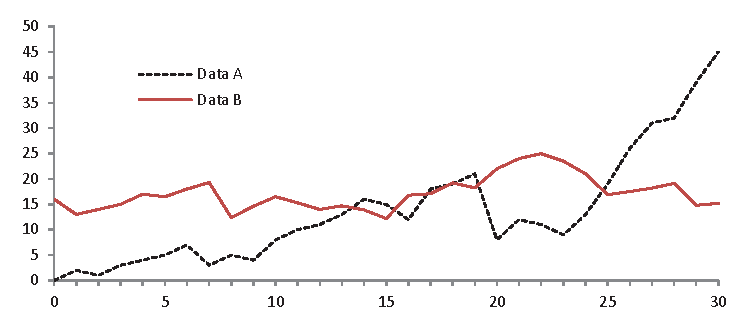
\includegraphics[width=\textwidth]{fig1.eps}
\caption{A figure caption is always placed below the illustration.
Please note that short captions are centered, while long ones are
justified by the macro package automatically.} \label{fig1}
\end{figure}

\begin{theorem}
This is a sample theorem. The run-in heading is set in bold, while
the following text appears in italics. Definitions, lemmas,
propositions, and corollaries are styled the same way.
\end{theorem}
%
% the environments 'definition', 'lemma', 'proposition', 'corollary',
% 'remark', and 'example' are defined in the LLNCS documentclass as well.
%
\begin{proof}
Proofs, examples, and remarks have the initial word in italics,
while the following text appears in normal font.
\end{proof}
For citations of references, we prefer the use of square brackets
and consecutive numbers. Citations using labels or the author/year
convention are also acceptable. The following bibliography provides
a sample reference list with entries for journal
articles~\cite{ref_article1}, an LNCS chapter~\cite{ref_lncs1}, a
book~\cite{ref_book1}, proceedings without editors~\cite{ref_proc1},
and a homepage~\cite{ref_url1}. Multiple citations are grouped
\cite{ref_article1,ref_lncs1,ref_book1},
\cite{ref_article1,ref_book1,ref_proc1,ref_url1}.
%
% ---- Bibliography ----
%
% BibTeX users should specify bibliography style 'splncs04'.
% References will then be sorted and formatted in the correct style.
%
% \bibliographystyle{splncs04}
% \bibliography{mybibliography}
%
\begin{thebibliography}{8}
\bibitem{ref_article1}
Author, F.: Article title. Journal \textbf{2}(5), 99--110 (2016)

\bibitem{ref_lncs1}
Author, F., Author, S.: Title of a proceedings paper. In: Editor,
F., Editor, S. (eds.) CONFERENCE 2016, LNCS, vol. 9999, pp. 1--13.
Springer, Heidelberg (2016). \doi{10.10007/1234567890}

\bibitem{ref_book1}
Author, F., Author, S., Author, T.: Book title. 2nd edn. Publisher,
Location (1999)

\bibitem{ref_proc1}
Author, A.-B.: Contribution title. In: 9th International Proceedings
on Proceedings, pp. 1--2. Publisher, Location (2010)

\bibitem{ref_url1}
LNCS Homepage, \url{http://www.springer.com/lncs}. Last accessed 4
Oct 2017
\end{thebibliography}
\end{document}




% old parts

% Meaning of CSI
%[From Halperin paper]
CSI captures signal strength and phase information for OFDM subcarriers and between each pair of transmit-receive antennas.
It runs on a commodity 802.11n NIC, and records Channel State Information (CSI) based on the 802.11 standard.
The CSI contains information about the channel between sender and receiver at the level of individual data subcarriers, for each pair of transmit and receive antennas.
%[From Halperin End]

% Structure of CSI
%[From HC's ELM paper]
In a frequency domain, the CSI of sub-carrier $\mathbf{c}$ between transmitter(Tx) and receiver(Rx) can be modeled as 
$\mathnormal{R}_{c} = \mathbf{H}_{c}\mathnormal{T}_{c} +\mathnormal{N}$ where the $\mathnormal{R}_{c}$ and $\mathnormal{T}_{c}$  denote the received and the transmitted signal vector of dimension $\mathnormal{r}$ and $\mathnormal{t}$, respectively. The $\mathnormal{N}$ is the additive channel noise and $\mathbf{H}_{c}$ is the $\mathnormal{r}\times\mathnormal{t}$ channel matrix. The CSI of sub-carrier $\mathnormal{c}$ can be modeled as follows:
\begin{equation}
    \mathnormal{h}_{c} = \mid\mathnormal{h}_{c}\mid\mathnormal{e}^{\angle\theta},
\end{equation}
where $\mid\mathnormal{h}_{c}\mid$ and $\theta$ represent the amplitude and the phase of the sub-carrier, respectively.
%[From HC's ELM end]


% description of siamese
In this paper, we propose a for signature verification system that is applicable for WIFI CSI signal, which is more complex and larger than handwritten images. 
% advantages of using Convnet filter
Based on Convnets as feature extractor, we are able to make feature vector from CSI signal reflecting local connectivity between signals at a near frequency range and closer measurement time. 
The proposed method achieved better performance because it is applicable to all points of CSI signals. This is due to the weight sharing the property of the Convnet filter.
